\documentclass[11pt,a4paper,oldfontcommands]{memoir}
\usepackage[utf8]{inputenc}
\usepackage[T1]{fontenc}
\usepackage{microtype}
\usepackage[dvips]{graphicx}
\usepackage{xcolor}
\usepackage{bookman}
\usepackage{graphicx,xcolor}
\usepackage[usestackEOL]{stackengine}
\usepackage[percent]{overpic}


\usepackage[
breaklinks=true,colorlinks=true,
%linkcolor=blue,urlcolor=blue,citecolor=blue,% PDF VIEW
linkcolor=black,urlcolor=black,citecolor=black,% PRINT
bookmarks=true,bookmarksopenlevel=2]{hyperref}

\usepackage{geometry}
% PDF VIEW
% \geometry{total={210mm,297mm},
% left=25mm,right=25mm,%
% bindingoffset=0mm, top=25mm,bottom=25mm}
% PRINT
\geometry{total={210mm,297mm},
left=20mm,right=20mm,
bindingoffset=10mm, top=25mm,bottom=25mm}

\OnehalfSpacing
%\linespread{1.3}

%%% CHAPTER'S STYLE
\chapterstyle{ell}
%\chapterstyle{ger}
%\chapterstyle{madsen}
%\chapterstyle{ell}
%%% STYLE OF SECTIONS, SUBSECTIONS, AND SUBSUBSECTIONS
\setsecheadstyle{\Large\bfseries\sffamily\raggedright}
\setsubsecheadstyle{\large\bfseries\sffamily\raggedright}
\setsubsubsecheadstyle{\bfseries\sffamily\raggedright}


%%% STYLE OF PAGES NUMBERING
%\pagestyle{companion}\nouppercaseheads 
%\pagestyle{headings}
%\pagestyle{Ruled}
\pagestyle{plain}
\makepagestyle{plain}
\makeevenfoot{plain}{\thepage}{}{}
\makeoddfoot{plain}{}{}{\thepage}
\makeevenhead{plain}{}{}{}
\makeoddhead{plain}{}{}{}


\maxsecnumdepth{subsection} % chapters, sections, and subsections are numbered
\maxtocdepth{subsection} % chapters, sections, and subsections are in the Table of Contents


%%%---%%%---%%%---%%%---%%%---%%%---%%%---%%%---%%%---%%%---%%%---%%%---%%%
\begin{document}

%%%---%%%---%%%---%%%---%%%---%%%---%%%---%%%---%%%---%%%---%%%---%%%---%%%
%   TITLEPAGE
%
%   due to variety of titlepage schemes it is probably better to make titlepage manually
%
%%%---%%%---%%%---%%%---%%%---%%%---%%%---%%%---%%%---%%%---%%%---%%%---%%%
\thispagestyle{empty}

{%%%
\sffamily

\centering
\Large

~\vspace{\fill}

{\huge 

\includegraphics{img/logo.png}\\
TOPLIS
}

\vspace{2.5cm}

{\LARGE
TopSky plugin for Portugal vACC
}

\vspace{3.5cm}

User Manual\\
Version 2.0\\

\vspace{\fill}

October 2022

%%%
}%%%

\cleardoublepage
%%%---%%%---%%%---%%%---%%%---%%%---%%%---%%%---%%%---%%%---%%%---%%%---%%%
%%%---%%%---%%%---%%%---%%%---%%%---%%%---%%%---%%%---%%%---%%%---%%%---%%%

\tableofcontents*

\clearpage

%%%---%%%---%%%---%%%---%%%---%%%---%%%---%%%---%%%---%%%---%%%---%%%---%%%
%%%---%%%---%%%---%%%---%%%---%%%---%%%---%%%---%%%---%%%---%%%---%%%---%%%

\chapter{Introduction}

\section{Disclaimer}
Although - as its name suggests - the plugin is based on TOPLIS and the TopSky ATM system, it is in no way affiliated with or endorsed by Thales Group or NAV Portugal. Similarities between plugin features and the real system are not entirely coincidental, but the plugin can not be used as a real world training aid. ~\cite{git}\\

\section{Foreword}
EuroScope, a controller client developed by Gergely Csernák for the VATSIM network, was first released for public use in September 2007. One of the biggest changes in version 3.1 was the possibility for the user community to customize the program to an even higher degree than was possible before by writing their own plugins that can be used to alter the way information is presented and even create completely new functionality into the program. This allowed creating very detailed simulations of all kinds of ATC systems without making the main program overly complex. Version 3.2 expands on these possibilities, making it possible to create even better plugins.
The TopSky plugin (a.k.a. The Plugin Formerly Known As “EUROCAT 2000 E”) started out as a very small project to create a couple of customized aircraft tag items, but as more information about the real system and the possibilities with the plugin development became available, it slowly grew to include an almost complete set of tag items, tag menus, graphical elements on the radar display and some additional functionality.

\chapter{System Description}
\section{Main Window}
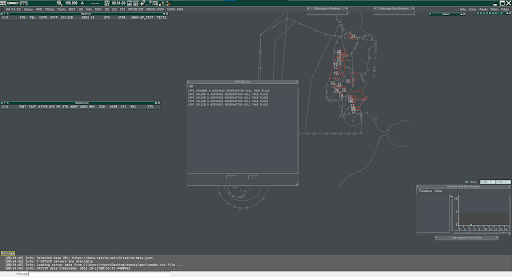
\includegraphics[width=15cm, keepaspectratio]{img/mainwindow.png}\\
Euroscope should load with some preplaced windows similar to the above configuration\\

Screen resolutions other than 1920x1080 will yield different results. Larger resolutions will bring preplaced windows towards the left and middle, while smaller resolutions may potentially place windows outside the screen. It is recommended for users experiencing difficulties related to their screen size to experiment and create custom settings in the TopSkySettingsLocal file containing revised window placements adjusted for their own screen. Refer to \texttt{\detokenize{TopSky_Developer_Guide_Settings.xlsx}} for available settings.\\

\section{Global Menu}

\includegraphics{img/globalmenu.png}\\
The Global Menu is located on the top edge of the radar screen. It displays the current UTC time and contains a number of submenus which are explained below.

\subsection{Setup Menu}
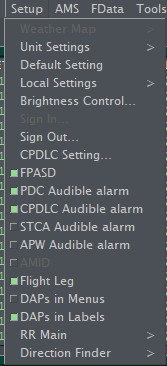
\includegraphics{img/Setup.png}\\
Setup Menu allows for various adjustments. Each position will load its defined settings based on the active Primary Frequency.\\ 
Most used options are CPDLC Setting for CPDLC operations and Default Setting to reset options.\\

\begin{tabular}{p{5cm}p{10cm}}
- Unit Settings > & Opens the Unit Settings submenu
\\- Default Setting & Resets all settings to their default values (keeps login callsign specific ones if they are active at the time). When clicked, a confirmation window will open, asking to confirm the reset.
\\- Local Settings > & Opens the Local Settings submenu
\\- Brightness Control > & Opens the Brightness Control Window
\\- Sign In… & Loads personal settings. The settings are specified in the \texttt{\detokenize{TopSkySettingsLocal.txt}} data file. When clicked, a confirmation window will open, asking to confirm the settings change.
\\- Sign Out… & Clears any personal settings and resets all settings to their default values. When clicked, a confirmation window will open, asking to confirm the settings change.
\\- CPDLC Setting… & Opens the CPDLC Setting Window
\\- FPASD & Toggles on/off the display of flight plan tracks
\\- PDC Audible alarm & Toggles on/off playing a sound for received PDC messages
\\- CPDLC Audible alarm & Toggles on/off playing a sound for received CPDLC messages
\\- STCA Audible alarm & Toggles on/off playing a sound for STCA alerts
\\- APW Audible alarm & Toggles on/off playing a sound for APW alerts
\\- AMID & Not implemented
\\- Flight Leg & Toggles on/off the automatic display of the Flight Leg for a specified time when a track becomes assumed
\\- DAPs in Menus & Toggles on/off the display of DAPs in menus
\\- DAPs in Labels & Toggles on/off the display of DAPs in track labels
\\- RR Main > & Opens the RR Main submenu
\\- Direction Finder > & Opens the Direction Finder submenu
  \end{tabular}

\subsection*{Unit Settings submenu}
This submenu can be used to change the units used in the plugin. Any changes to the settings are session-
specific only, so they will be lost when exiting EuroScope.

\begin{tabular}{p{5cm}p{10cm}}
    \\- Altitude & Selects the units used for altitudes and vertical rates
    - Nautical (feet, feet per minute)
    - Metric (meters, meters per second)
    \\- Flight level & Selects the units for flight levels – only applicable with metric altitudes
    - Nautical (hundreds of feet)
    - Metric (meters)
    \\- Distance & Selects the units used for distances
    - Nautical (nautical miles)
    - Metric (kilometers)
    \\- Speed & Selects the units used for speeds
    - Nautical (knots)
    - Metric (kilometers per hour)
\end{tabular}

\subsection*{Local Settings submenu}
This submenu allows changing some of the plugin’s settings. Any changes to the settings are session-
specific only, so they will be lost when exiting EuroScope.

\begin{tabular}{p{5cm}p{10cm}}
\\- Vertical reference    & Selects the pressure reference to be used at or below the
transition altitude:
• QNH Altitude above mean sea level
• QFE Height above the aerodrome elevation
(set/check it in the adjacent box)
\\- Used equipment codes  & Selects whether to use or disregard the equipment codes
found in the flight plans:
• All Use all codes
• ICAO Use all codes when specified in ICAO format
• ICAO-alt As ICAO, but force transponder to report altitude
• None Disregard all codes

\\- ASSR codes    & Selects the transponder code source:
• Plugin Plugin data file (reverts to ESE if no codes found)
• ESE ESE file
• Range Fixed code range
\\- Groundspeed   & Selects whether to use pilot client reported ground speed or a
plugin calculated value. Normally the reported value should be
used as it is more accurate and stable, but some clients report
wrong values. If that causes problems, you can try selecting the
plugin calculated value instead
\\- Transfer confirmation & Selects when to display the Transfer Confirmation Window:
• On Always when CFL is not equal to XFL
• NotRFL When CFL is not equal to XFL unless XFL = RFL
• Off Never, any CFL value is OK
\\- CFL menu default value    & Selects the default value for the CFL menu when it is opened:
• XFL FSS or CTR: RFL if not yet reached, otherwise as below
Other: The XFL value, or current CFL value with no XFL
• CFL The current CFL value
• RFL The RFL value
\\- FPCP inhibit  & FPCP calculations start when tracks are within this time from
entering active sector
\\- STCA alert    & Selects which aircraft display the STCA alert:
• All All aircraft
• Own+Co Only assumed and coordinated aircraft
• Own Only assumed aircraft
\\- STCA alert sound  & Selects which STCA alerts trigger the alert sound:
• All All alerts
• Own+Co Only alerts with assumed and/or coordinated
aircraft involved
• Own Only alerts with assumed aircraft involved
\\- APW alert & Selects which aircraft display the APW alert:
• All All aircraft
• Own+Co Only assumed and coordinated aircraft
• Own Only assumed aircraft
\\- APW alert sound   & Selects which STCA alerts trigger the alert sound:
• All All alerts
• Own+Co Only alerts for assumed or coordinated
aircraft
• Own Only alerts for assumed aircraft
\\- METAR source  & Selects the METAR data source for the plugin windows that
display METAR data
\\- FPASD filter  & Allows filtering of displayed FPASD tracks based on sector state
• Coord Display tracks at least in the coordinated state
• Conc Display tracks at least in the concerned state
• None Display all tracks

\end{tabular}

\subsection*{RR Main submenu}
\begin{tabular}{p{5cm}p{10cm}}
    - [] Rings On/Off & Toggles the range rings on/off
    \\- Point & Sets the rings centerpoint. Either click on the radar screen or
    enter the desired point in the text field. Fixes, VORs, NDBs and
    airports from the active sector file can be used as well as
    coordinates in the flight plan format (DD[N/S]DDD[E/W] or
    DDMM[N/S]DDDMM[E/W], e.g. 60N025E or 0811S00300W).
    Entering an empty text string resets the rings to be shown at
    the radar screen centerpoint.
    \\- Separation & Sets the separation between adjacent rings
    \\- Number & Sets the number of rings drawn
    \\- [] Highlight & Toggles highlight (drawn with solid line) of specified rings
    \\- Step & Sets interval of highlighted rings
\end{tabular}

\subsection*{Direction Finder submenu}
Not operational.

\subsection{AMS menu}
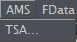
\includegraphics{img/AMS.png}\\
Opens the \textit{\titleref{menu:tsa}}.

\subsection{FData menu}
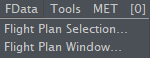
\includegraphics{img/FData.png}\\
Opens the \textit{\titleref{menu:fpsel}} and \textit{\titleref{menu:fpwin}}.

\subsection{Tools menu}

\subsection{Tools menu}
%TODO\includegraphics{img/tools.png}\\
\begin{tabular}{p{5cm}p{10cm}}
\\- Flight Plan Lists > & Opens the Flight Plan Lists submenu
\\- CARD… & Opens the \textit{\titleref{win:card}}
\\- SAP… & Opens the \textit{\titleref{win:sap}}
\\- Vertical Aid Window… & Opens the \textit{\titleref{win:vaw}}
\\- Message In… & Opens the \textit{\titleref{win:mi}}
\\- Message Out… & Opens the \textit{\titleref{win:mo}}
\\- CPDLC > & Opens the CPDLC submenu
\\- LAT/LONG… & Opens the \textit{\titleref{win:cur}}
\end{tabular}

\subsection*{Flight Plan Lists submenu}
\begin{tabular}{p{5cm}p{10cm}}
    - [] List options bar           & Toggles the display of list options on the Global Menu
    \\- Sector List…                & Opens the Sector List
    \\- [] Informed                 & Toggles the display of informed aircraft
    \\- [] Concerned                & Toggles the display of concerned aircraft
    \\- [] Redundant                & Toggles the display of redundant aircraft
    \\- Load Factor List…           & Opens the \textit{\titleref{list:lf}}
    \\- ETWR List…                  & Opens the \textit{\titleref{list:etwr}}
    \\- <adep>                      & ETWR List departure airports filter
    \\- Uncont. List 1…             & Opens the \textit{\titleref{list:ul1}}
    \\- <filter>                    & Uncontrolled 1 List state filter
    \\- <units>                     & Uncontrolled 1 List units filter
    \\- Uncont. List 2…             & Opens the \textit{\titleref{list:ul2}}
    \\- <filter>                    & Uncontrolled 2 List state filter
    \\- <units>                     & Uncontrolled 2 List units filter
    \\- Lost List…                  & Opens the \textit{\titleref{list:ll}}
    \\- Resectorisation List…       & Opens the \textit{\titleref{list:rl}}
    \\- <lfunc>                     & Resectorisation List LFUNC filter
    \\- Traffic Mgmt. List 1…       & Opens the \textit{\titleref{list:tml1}}
    \\- <state>                     & Traffic Management List 1 flight plan state filter
    \\- <ades>                      & Traffic Management List 1 destination airports filter
    \\- <via>                       & Traffic Management List 1 route points filter
    \\- Traffic Mgmt. List 2…       & Opens the \textit{\titleref{list:tml2}}
    \\- <state>                     & Traffic Management List 2 flight plan state filter
    \\- <ades>                      & Traffic Management List 2 destination airports filter
    \\- <via>                       & Traffic Management List 2 route points filter
\end{tabular}\\

When enabled, the list options bar displays “Info Conc Redu Filter Filter” on the right edge of the Global
Menu. The first three toggle the respective settings for the Sector List and are colored with the appropriate
color when enabled, and the last two are displayed in “VFR” color when the corresponding
Uncontrolled list is somehow filtered. Clicking on them opens the Flight Plan Lists submenu to change
the filtering options.\\
Left-clicking <filter> cycles through “ALL” (no filtering), “ON-CONTACT” (only tracks on-contact with
anyone), “ON-CONTACT-PPOS” (only tracks on-contact with you) and “FREE” (only tracks in the free state).\\
Left-clicking <units> opens a text entry box to enter a comma-separated list of aerodrome ICAO codes to
filter the list. When entered, the list will display a flight only if one of the entered codes is its departure or
destination, or the code is found in its scratchpad (OP-TEXT2).\\

Left-clicking <lfunc>, <adep>, <ades> and <via> open text entry boxes to enter comma-separated lists for
controlled ID’s, ICAO codes and point names respectively to filter the affected lists.\\
Left-clicking <state> toggles between “ALL” (no filtering), “SIMUL+TERM” (not started flight plans filtered),
“NOTST+SIMUL” (terminated flight plans filtered) and “SIMUL” (not started and terminated flight plans
filtered).\\

\subsection*{CPDLC submenu}
\begin{tabular}{p{5cm}p{10cm}}
- Microphone Check      & Opens the \textit{\titleref{win:dlmcm}}
\\- Current Messages…   & Opens the \textit{\titleref{win:dlcmw}}
\\- History Messages…   & Opens the \textit{\titleref{win:dlhmw}}
\end{tabular}\\

\subsection{MET menu}
\begin{tabular}{p{5cm}p{10cm}}
- Messages… & Opens the \textit{\titleref{win:wxcmw}}
\\- QNH/TL    & Opens the \textit{\titleref{win:wxqnh}}
\end{tabular}\\

\subsection{[0]}
Not implemented (always shows a zero value).

\subsection{Info menu}
\begin{tabular}{p{5cm}p{10cm}}
- General Information…      & Opens the \textit{\titleref{win:gi}}
\\- Document Viewer…          & Opens the \textit{\titleref{win:dv}}
\\- NOTAM…                    & Opens the \textit{\titleref{list:notam}}
\\- Aerodrome…                & Opens the \textit{\titleref{menu:ad}}
\\- LFUNC Frequency Plan…     & Opens the \textit{\titleref{win:lfunc}}
\\- [] Airport labels         & Toggles airport labels selection
\\- [] Fix labels             & Toggles fix labels selection
\\- [] NDB labels             & Toggles NDB labels selection
\\- [] VOR labels             & Toggles VOR labels selection
\end{tabular}\\
When holding <ALT>, text labels will be displayed for airports, fixes, NDBs
and VORs when the mouse cursor is placed over them. When one or more of the categories in the Info
menu is selected, only those categories will display the labels. The “Label” buttons open submenus to select
what information is shown on the corresponding labels. All the information is from the active sector file.\\

\subsection{MSG menu}
\begin{tabular}{p{5cm}p{10cm}}
- Notepad…              & Opens the \textit{\titleref{win:notepad}}
\\- Personal Queue…     & Opens the \textit{\titleref{win:pq}}
\\- ATC Messages…       & Opens the \textit{\titleref{win:atcm}}
\\- Prim Freq Messages… & Opens the \textit{\titleref{win:pfm}}
\\- NAT Track Messages… & Opens the \textit{\titleref{win:natm}}
\\- Text notes >        & Opens the Text notes submenu
\end{tabular}\\

It is possible to insert text notes on the radar screen to act as reminders. They will stay fixed at the
geographical coordinates they are inserted to, the coordinates defining the center point of the note.
\\When creating a note, a text entry field opens to enter the note text. When the [Enter] key is pressed, the
note will be created at the current mouse cursor position.
\\The notes can be deleted one by one or all of them at the same time. When deleting one by one, the notes
are boxed to display their click areas. Clicking on one will delete the note. Pressing the [Esc] key or selecting
the “Delete...” menu item again will abort the operation.

\subsection*{Text notes submenu}
\begin{tabular}{p{5cm}p{10cm}}
\\- Create…     & Creates a new text note
\\- Delete…     & Deletes a single text note
\\- Delete all  & Deletes all text notes
\end{tabular}\\

\subsection{[x]}
Shows the number of high priority messages in the personal message queue. These are critical failures in
the plugin code. Open the Personal Queue Window to view the messages. The number is limited to 99, and
is shown on “Global Menu Highlight” background when the window is not open.

\subsection{[x]}
Shows the number of low priority messages in the personal message queue. These are warnings about
invalid data in the plugin data files. Open the Personal Queue Window to view the messages or see the
Plugin Status submenu for more detailed information on the problem(s). The number is limited to 99, and is
shown on “Global Menu Highlight” background when the window is not open.

\subsection{STS menu}
\begin{tabular}{p{5cm}p{10cm}}
- Plugin Status >                & Opens the Plugin Status submenu
\\- Safety Nets Status…            & Opens the \textit{\titleref{win:sn}}
\\- Divergence Detection Status…   & Opens the \textit{\titleref{win:dds}}
\\- MTCD Status…                   & Opens the \textit{\titleref{win:mtcds}}
\\- CPDLC Default Status [ON/OFF]  & Toggles the CPDLC Default Status On/Off
\\- Runway In Use                  & Opens the \textit{\titleref{menu:ad}}
\\- Supervisory >                  & Opens the Supervisory submenu
\\- RWY line display…              & Opens the \textit{\titleref{menu:ad}}
\end{tabular}\\

\subsection*{Plugin Status submenu}
Shows the version of the plugin as well as some information on the loaded data files. Each data file reports
its state with one of the following indicators:\\
\begin{tabular}{p{5cm}p{10cm}}
- OK        & File contains usable information and no faults
\\- NO DATA   & File not found or contains no usable information
\\- BAD DATA  & File contains invalid data (in “Warning” color)
\end{tabular}\\
Depending on the file, there are one to three of the following buttons available:\\
\begin{tabular}{p{5cm}p{10cm}}
- Reload                    & Reloads the data file
\\- View                    & Displays the data in the file on the radar display
\\- Save (Areas)            & Saves a snapshot of the current area activation data
\\- Save set (Maps \& MapsL) & Saves a list of currently active radar screen specific maps
\\- Load set (Maps \& MapsL) & Loads a saved list of active screen specific maps
\end{tabular}\\ 

Left-clicking the Save button will save the currently set manual activation periods as well as the
information if an area with automatic schedules is set to manual mode. The information is saved to the
“TopSkyAreasManualAct.txt” file in the same folder as the plugin dll. If the file already exists, the plugin will
ask for confirmation as the save operation will overwrite any existing data.\\
Depending on the maps data file setup, the display state of some or all of the maps may be specific to each
radar screen. The Save set and Load set functions can be used to transfer the display state of these maps
from one radar screen to another.\\
Right-clicking the Reload button for Settings \& SettingsL has a special purpose. It opens a text entry box to
type in a callsign whose settings should be loaded instead of the real login callsign. When entered, the
callsign will be displayed next to the “Reload” button, and whenever a VATSIM callsign change is detected,
an information popup is displayed to remind that the plugin settings are still forced to the manually
entered callsign. This feature can be used for example to use settings for different positions on different
EuroScope instances when providing top-down services, or to use settings for a specific position when
logged in with an observer/staff/supervisor callsign. Clearing the entered callsign reverts to using the
settings based on the actual login callsign.\\

\subsection*{Supervisory submenu}
\begin{tabular}{p{5cm}p{10cm}}
- Operations Rate...     & Opens the \textit{\titleref{win:or}}
\\- Predicted Traffic... & Opens the \textit{\titleref{win:pt}}
\end{tabular}\\ 

\subsection{RRxxx/Off}
Opens the \textit{\titleref{menu:rr}}. If the rings are selected on,
“xxx” displays the distance between consecutive rings, otherwise “Off”.

\subsection{Mxxx-yyy}
Displays the status of the filters. If any filter is enabled and Quick Look is not toggled on, the color of the
text is “Global Menu Highlight”.\\
Only the altitude filter status is shown. “xxx” displays the Lower filter value and “yyy” the Upper filter
value, in hundreds of feet.\\

\subsection{S000-999}
Not implemented (shows static values).\\

\section{Track Presentation}

\section{Track Label Menus}

\section{Flight Leg}

\section{Windows}

\subsection{Airspace Management Window}
\label{menu:tsa}
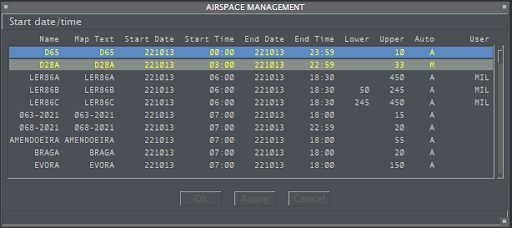
\includegraphics{img/tsa.png}\\
This window is used for the activation and deactivation of the areas for the APW and SAP functionality. Each area can have a start time and/or an end time defined for its activation, or it can be activated without any time limits, making it active until deactivated manually. Additionally, lower and upper altitude limits are given. An area can have activation schedules defined in the area data file. Such areas will be automatically activated as long as their “Auto” option is selected ( “A” in the “Auto” column). The “Auto” option cannot be selected for areas that don’t have an activation schedule defined in the area data file.

Dates will be shown in the format “yymmdd” and times in “hh:mm” and they must be entered in the same format. Entering an empty string for a date will clear it and the related time value and vice versa. When entering a time or date value to an empty field, the other value is automatically set to the current time/date value. Entering an empty string to the Map Text, Lower or Upper fields will reset the value to the default one from the data file.

Altitudes are shown in hundreds of feet if at or below the transition altitude, otherwise in flight levels. They must be entered in the same format.

An area’s activation status can be inactive, pre-active or active. A pre-active area is an area that will become active within 30 minutes and is shown in yellow text on a gray background. An active area is shown with yellow text on a blue background. The APW system will not alert for a pre-active area, but for the SAP system a pre-active area is considered as being active.

The mouse click areas of the Airspace Management Window:
\begin{itemize}[\textbullet] 
    \item Sorting option text (e.g. “Start date/time”) Opens a pop-up menu to select a sorting option for the list 
    \item Right-click to open an area pop-up menu
    \item Other fields Left-click to edit field (when edit function active)
    \item “Ok” button Applies the changes, closes the window
    \item “Apply” button Applies the changes
    \item “Cancel” button Cancels the changes 
\end{itemize}

The sorting pop-up menu contains the following items:
\begin{itemize}[\textbullet] 
    \item Start Date Sorts based on the Start Date/Time, earliest first
    \item Name Sorts alphabetically based on the Name field
    \item Map Text Sorts alphabetically based on the Map Text field 
\end{itemize}
With the area pop-up menu opened, the area text row background changes to black. The menu contains the following items:
\begin{itemize}[\textbullet] 
    \item ACTIVATE Clears any activation times and activates the area
    \item DEACTIVATE Clears any activation times and deactivates the area
    \item AUTO If an activation schedule is found in the area data file, sets the
    \item area to be activated automatically
    \item VALIDATE Not implemented
    \item EDIT Allows to change the area parameters
    \item COPY Not implemented
    \item DELETE Clears any activation times, returns label and altitude limits to their default values and deactivates the area
\end{itemize}
After any selection from the pop-up menu, “Ok”, “Apply” or “Cancel” must be selected to apply or cancel the selection. 

Preactive and active areas are displayed on the radar screen. The area border is drawn using a predefined color and it may be filled as well. A predefined text label may also be displayed, showing information about the area. A very small “+” symbol will be drawn at that location. By holding the left mouse button down on that symbol, a full area label will be displayed, showing:

\begin{center}
        Name\\ 
        Map text\\
        Upper level limit\\
        Start time --------- End time\\
        Lower level limit\\time in minutes until the area becomes active
\end{center}

\section{Lists}

\subsection{NOTAM List}
\label{list:notam}
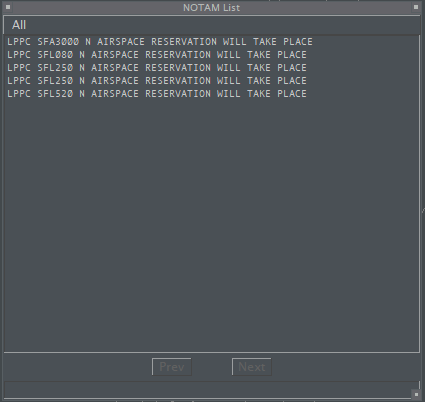
\includegraphics{img/notamlist.png}\\
The NOTAM List is automatically displayed at startup in order to fetch the current FUA. It may be closed after loading.\\

\section{Safety Nets}

\section{Monitoring Aids}

\section{Flight Plan Conflict Probe}

\appendix

\chapter{Label field descriptions}

\chapter{Color Values}

\chapter{Keyboard Shortcuts}

\bibliographystyle{unsrt}
\bibliography{refs}

\end{document}

